\newpage
{\bfseries ҒТАМР 50.43.15}

{\bfseries ЖОЛ ҚИЫЛЫСТАРЫНДАҒЫ КӨЛІК ҚҰРАЛДАРЫНЫҢ АҒЫНЫН НАҚТЫ УАҚЫТ
РЕЖИМІНДЕ ДИНАМИКАЛЫҚ РЕТТЕУ}

{\bfseries \textsuperscript{1}Д.С. Жамангарин, \textsuperscript{1}С.А.
Алтынбек, \textsuperscript{1}А.Д. Тулегулов\textsuperscript{🖂},}

{\bfseries \textsuperscript{1}К.М. Акишев, \textsuperscript{2}Н.П.
Сапарходжаев}

\textsuperscript{1}Қ. Құлажанов атындағы Қазақ технология және бизнес
университеті, Астана, Қазақстан,

\textsuperscript{2}Д. Серікбаев атындағы Шығыс Қазақстан техникалық
университеті., Өскемен, Қазақстан

\textsuperscript{🖂}Корреспондент-автор: tad62@ya.ru

Соңғы жылдары қалалық жерлерде бағдаршамдардың өткізу қабілеттілігін
арттыру мақсатында көлік құралдарының кептелісін динамикалық басқаруға
көбірек көңіл бөлінуде. Осы мақсатта кіру жылдамдығына негізделген жеке
traf C шамдары үшін бірқатар адаптивті басқару алгоритмдері ұсынылды.
Алайда, нақты уақыт режимінде бірнеше қиылыстардан өтетін жол
жағдайларын ескере отырып, бағдаршамдардың өткізу қабілеттілігін арттыру
мәселесіне көңіл бөлінді. Бұл жұмыста біз әр түрлі шығыс бағыттарына
кіретін көліктерді қарастыра отырып, максималды өткізу мәселені
тұжырымдаймыз. Содан кейін біз жаңа адаптивті traf C жарық сигналын
басқару алгоритмін ұсынамыз, ол жол қозғалысын барынша арттыруға және
қиылыста көлік құралдарының күту уақытын қысқартуға мүмкіндік береді.
Ұсынылған алгоритм негізгі және көршілес қиылыстардың нақты уақыттағы
жол жағдайына байланысты traf C жарық сигналының фазалары мен ұзақтығын
реттейді. SUMO модельдеу арқылы біз ұсынылған алгоритмнің өткізу
қабілеттілігі мен орташа жүру уақыты тұрғысынан тиімділігін көрсетеміз.

{\bfseries Түйін сөздер:} адаптивті жүйелер, traf C, адаптивті басқару,
алгоритм, SUMO модельдеу.

{\bfseries ДИНАМИЧЕСКОЕ РЕГУЛИРОВАНИЕ ПОТОКА ТРАНСПОРТНЫХ СРЕДСТВ НА
ПЕРЕКРЕСТКАХ В РЕЖИМЕ РЕАЛЬНОГО ВРЕМЕНИ}

{\bfseries \textsuperscript{1}Д.С. Жамангарин, \textsuperscript{1}С.А.
Алтынбек, \textsuperscript{1}А.Д.
Тулегулов}\textsuperscript{🖂}{\bfseries ,}

{\bfseries \textsuperscript{1}К.М. Акишев, \textsuperscript{2}Н.П.
Сапарходжаев}

\textsuperscript{1}Казахский университет технологии и бизнеса имени К.
Кулажанова, Астана, Казахстан,

\textsuperscript{2}Восточно-Казахстанский технический университет им. Д.
Серикбаева,

Усть-Каменогорск, Казахстан,

e-mail: tad62@ya.ru

В последние годы все больше внимания уделяется динамическому управлению
заторами транспортных средств с целью увеличения пропускной способности
светофоров в городских районах. С этой целью был предложен ряд
алгоритмов адаптивного управления для отдельных ламп traf C, основанных
на скорости входа. Однако с учетом дорожных условий, проходящих через
несколько перекрестков в режиме реального времени, внимание было уделено
вопросу увеличения пропускной способности светофоров. В данной статье мы
формулируем проблему максимальной пропускной способности, рассматривая
транспортные средства, въезжающие в разные направления. Затем мы
представляем новый адаптивный алгоритм управления световым сигналом traf
C, который позволяет максимизировать дорожное движение и сократить время
ожидания транспортных средств на перекрестке. Предлагаемый алгоритм
регулирует фазы и продолжительность светового сигнала traf C в
зависимости от дорожной ситуации в реальном времени между основным и
соседним пересечениями. С помощью моделирования SUMO мы демонстрируем
эффективность предложенного алгоритма с точки зрения пропускной
способности и среднего времени в пути

{\bfseries Ключевые слова}. адаптивные системы, traf C, адаптивное
управление, алгоритм, моделирование SUMO.

{\bfseries DYNAMIC CONTROL OF THE FLOW OF VEHICLES AT INTERSECTIONS IN REAL
TIME}

{\bfseries \textsuperscript{1}D. Zhamangarin, \textsuperscript{1}S.
Altynbek, \textsuperscript{1}A. Tulegulov}\textsuperscript{🖂}{\bfseries ,
\textsuperscript{1}K. Akishev, \textsuperscript{2}N. Saparkhodzhaev}

\textsuperscript{1}K. Kulazhanov Kazakh University of Technology and
Business, Astana, Kazakhstan

\textsuperscript{2}D. Serikbayev East Kazakhstan Technical University,
Ust-Kamenogorsk, Kazakhstan

e-mail: tad62@ya.ru

In recent years, more and more attention has been paid to dynamic
traffic congestion management in order to increase traffic light
capacity in urban areas. To this end, a number of adaptive control
algorithms have been proposed for individual traf C lamps based on the
input speed. However, taking into account the road conditions passing
through several intersections in real time, attention was paid to the
issue of increasing the traf C light capacity. In this article, we
formulate the problem of maximum throughput by considering vehicles
entering in different directions. Then we present a new adaptive traffic
light control algorithm that maximizes traf C and reduces the waiting
time for vehicles at the intersection. The proposed algorithm adjusts
the phases and duration of the traf C light signal depending on the
real-time road conditions of the main and adjacent intersections.
Through SUMO simulations, we demonstrate the effectiveness of the
proposed algorithm in terms of bandwidth and average travel time.

{\bfseries Key words.} adaptive systems, traf C, adaptive control,
algorithm, SUMO modeling.

{\bfseries Кіріспе.} Мегаполистерде урбанизацияға байланысты белгілі бір
жолдардағы автокөлік тығыздығы жоғары қарқынмен өсті. Бұл жолдың
кептелуіне, апаттарға, жанармай шығынына, СО шығарындыларына және
трафиктің кешігуіне әкелді {[}1,2{]}. Бұл мәселелер зерттеу жұмыстарының
назарын арттыруға түрткі болды және көлік қозғалысын басқарудың әртүрлі
стратегияларын әзірлеуге әкелді. Пайда болған стратегиялардың
бірі-қауіпсіздік камералары, traf C бейнекамералары, пьезоэлектрлік
датчиктер, индуктивті ілмектер және т.б. сияқты әртүрлі сенсорлық
технологияларды қолдану арқылы жиналған ақпаратқа сүйенетін
интеллектуалды көлік жүйесі ұғымын жүзеге асыру, жол жағдайын бақылау
және автокөлік жүргізушілерін сигналдары арқылы ескертуге болады.
Алайда, ITS-де қолданылатын бақылаудың мұндай әдеттегі әдістері шектеулі
қамту мен техникалық қызмет көрсетудің жоғары құнына байланысты тиімді
болмайды. Осы кемшіліктерді жою және нақты уақыт режимінде трафиктің
нақты деректерін жинау үшін ITS тұжырымдамасы сымсыз байланыс
технологияларымен толықтырылған, бұл көлік құралдарының арнайы желісінің
дамуына әкеледі. Сонымен қатар, traf C жарықтандыру уақытын жақсарту
үшін сымсыз сенсорлық желілер пайдаланылды {[}3,4{]}.

{\bfseries Материалдар мен әдістер.} Қалалық жолдардағы С қозғалысының
жағдайын жақсартуға арналған танымал VTM стратегияларын екі топқа бөлуге
болады. Бірінші топ traf C деректерін жинауға, пайдалануға және деректер
негізінде көліктерді айналып өтетін қайта бағыттау алгоритмдерін
қолдануға бағытталады {[}5,6{]}. Сонымен қатар, зерттеулер әрбір жолдың
нақты уақыттағы қозғалыс жағдайларын ескеруге мүмкіндік беру үшін сымсыз
байланыс технологиялары мен есептеу ресурстарындағы жетістіктерді
пайдалана отырып, traf C адаптивті басқаруды зерттейді {[}7,8{]}.
Зерттеу жұмыстарының көпшілігінің негізгі бағыты негізінен бір қиылысты
қиылыстыра отырып, traf C өткізу қабілетін арттыруға бағытталған; тек
бірнеше зерттеулер traf C максимизациясы үшін бірнеше қиылыстарды
қарастырады {[}9,10{]}. Алдыңғы жұмыстардан айырмашылығы, бұл жұмыс
мақсатты қиылыстағы және оның төрт бағыттағы көршілес қиылыстарындағы
нақты уақыттағы жағдайды ескере отырып, көлік құралдарының трафигін
максимизациялау мәселесін қарастырады және TFM - ді максималды бүтін сан
ретінде модельдейді.

Әдетте кептеліс тудыратын жол желісіне кіретін көлік құралдары әр түрлі
шығыс бағыттармен жүруге ниетті болғандықтан, кіру және шығу нүктелері
бірдей көлік құралдарының ағыны 0 және 1 желісіндегі геокартаға
түсірілуі мүмкін. Сонымен қатар, бір 0-ға жататын көлік құралдарының
саны, яғни шығу және келу позициялары бірдей көлік құралдары тобы
белгілі бір аралықтын сұранысына сәйкес келуі мүмкін. Біз жол желісін
gd(V;E) бағытталған графигі түрінде ұсынылған 0 желісіне геокартаға
түсіреміз, мұнда V және E сәйкесінше барлық қиылыстар мен жол
сегменттерін қамтиды. G-ге сүйене отырып, біз қарастырылған мәселесін
қуаттылық, 0 сигналдың уақыт үнемдеу және сұранысты қанағаттандыру
шарттарымен MCF-мен салыстыруға болатындығын көрсетеміз. Содан кейін біз
1-ші қиылысынан белгілі бір бағытқа қарай жасыл шамды күтіп тұрған
көліктерді ескере отырып, MCF үлгісін тұжырымдаймыз .

Қалыптасқан MCF мәселесін шешу үшін біз кептеліс пен бос жасыл ұзақтықты
азайту құралы ретінде бірнеше қиылыстардың(атомдардың) жол жағдайларын
ескеретін адаптивті traf C жарық фазасы мен ұзақтығын оңтайландыру
алгоритмін енгіземіз. Негізінде, traf C өткізу қабілеттілігін арттыруға
және қиылыста және оның қиылыстарында күту уақытын қысқартуға тырысады.
Сонымен қатар, трафиктің өткізу қабілеттілігінің артуы және күту
уақытының қысқаруы жергілікті және көршілес қиылыстардың айналасындағы
жолдардың қозғалыс деңгейін ескере отырып, динамикалық түрде реттеледі
және теңестіріледі. Traf C деректерін жинау үшін көлік құралдарындағы
борттық қондырғылар, Iare - дегі I жол бойындағы бөлімшелердегі (Rsu)
Obu және жол бойындағы қондырғылар (Rsu) арасындағы әртүрлі
коммуникациялық технологиялар пайдаланылады. Kіретін көліктердің саны,
барлық бағыттарды күту уақыты және т. б. сияқты i-дегі traf C
статистикасын бақылау.

Traf C деректері негізінде алынған кептеліс деңгейіне сүйене отырып,
өтіп бара жатқан көліктердің санын көбейту мен i - де орташа күту
уақытын қысқарту арасындағы тепе-теңдікті сақтау үшін traf C жарықты
басқарудың әртүрлі тәсілдерін қолданады.

Aвтокөлік туралы деректер негізінде алынған кептеліс деңгейіне сүйене
отырып, өтіп бара жатқан көліктердің санын көбейту мен i - де орташа
күту уақытын қысқарту арасындағы тепе-теңдікті сақтау үшін C
трафигіндегі жарықты басқарудың әртүрлі тәсілдерін қолданады. Tрафигінің
төмен көлемі байқалған кезде, күту уақытын қысқарту үшін бос жасыл
уақытты жоюға назар аударады. Сонымен қатар, С автокөліктің қарқынды
жағдайында назары жақын маңдағы жолдардағы кептелістерді азайтуға
бағытталған. Екі жағдайда да traf C жарық циклін реттеуді және/немесе
жергілікті және жақын маңдағы қиылыстардағы бақыланатын traf C деректері
негізінде жасыл жарық фазаларын және олардың ұзақтығын таңдау мен ретке
келтіруді оңтайландыруды таңдайды. Модельдеу нәтижесінде атомның
трафиктің өзгеруіне және өткізу қабілеттілігіне және пайдаланушының
кідірісіне бейімделудегі тиімділігі артады.

\emph{Aдаптивті бағдаршамды оңтайлату тәсілі}

АБОТ-тың басты ерекшелігі-жолдағы көлік құралдарының тығыздығының
динамикалық өзгеруіне байланысты traf c оңтайландырудың екі түрлі
тәсілін қолданылады. Тraf c жарық агентінен тұрады, атап айтқанда traf c
бақылаушысы және бағалаушы (TFW) және traf c жарық сигналын реттегіш
болады. Бағдаршам параллель жұмыс істейді және бір уақытта 1-суретте
көрсетілгендей бір-бірімен байланысады.

\begin{figure}[H]
	\centering
	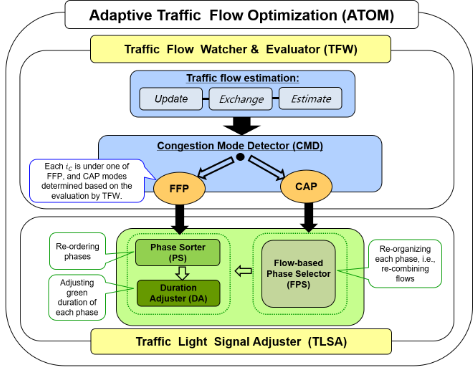
\includegraphics[width=0.5\textwidth]{assets/158}
	\caption*{\bfseries 1 --сурет. ЕКІ агент арасындағы өзара байланыс}
\end{figure}


ATOM traf C жалпы өткізу қабілетін жақсартуды және i-де күтілетін
көліктің орташа өткізу қабілетін азайтуды таңдайды. АБОТ екі жұмыс
істейді, атап айтқанда TFW және TLSA.

TFW жергілікті және жақын маңындағы қиылыстардағы С трафигінің
динамикалық өзгерістерін бақылайды және i бағытында келе жатқан С
трафигінің көлемін, сондай-ақ i-ден шығатын жолдардағы жағдайларды
бағалайды. Деректерді жинауды жол датчиктері, 802.11 p, 802.16, яғни
WiMAX немесе LTE-V немесе 3gpp Cellular-V2X(C-V2X) сияқты ӘРТҮРЛІ V2V,
V2I және I2I технологияларын қолдану арқылы іс жүзінде жүзеге асыруға
болады. Содан кейін TFW бақыланатын жолдағы кептеліс деңгейін бағалайды.
Негізінде, tfw кептелу режимінің детекторы (CMD) i күйін екі режимге
жіктейді, атап айтқанда, бос 0 кезеңі (FFP) және үздіксіз реттелетін
кезең. Сонымен қатар, TFW жүргізетін traf c оңтайландыруының әсерін
мезгіл-мезгіл аңықтап және өнімділікті жақсарту үшін нәтижелерді TLSA-ға
қайтарады. Сонымен қатар, TLSA төменде түсіндірілгендей, TFW бағалаған
i-дегі кептеліс деңгейіне байланысты әртүрлі стратегияларды қолдану
арқылы бағдаршамды оңтайландырады.

Бұл i-де қалатын немесе өтетін көлік құралдарының жалпы көлемі аз
болатын уақыт кезеңін анықтап, осылайша i-дегі traf c өткізу
қабілеттілігі негізінен циклдің ұзақтығына әсер етеді, оның барысында
әрбір кем дегенде бір рет жасыл шамға ауысады. FFP-де, әдетте, i-ден әр
түрлі бағытта өтетін көліктердің орташа күту уақытын қысқарту үшін қысқа
циклға артықшылық беріледі, өйткені i қызмет көрсететін көліктердің
жалпы саны аз. Сондықтан, FFP кезінде TLSA, бұдан әрі TLSA деп
белгіленеді, traf c жарық циклінің сәйкес ұзындығын есептейді мен онда
барлық F бір рет жасыл шаммен сақталады және жасыл сигналдың реті мен
ұзақтығын салыстырмалы түрде көп кіретін бағыттарға қолайлы етіп
реттейді. Сонымен қатар, FFP цикл ұзақтығын, фазаларын және жасыл
жарықтың ұзақтығын кезең - кезеңімен реттеуге байланысты үш ішкі
деңгейге бөлінеді.

Уақыт сигналдары симуляция арқылы тексеріледі.

\emph{Симуляциялық орта және тиімділік көрсеткіштері}

Модельдеу Python тілінде SUMO көмегімен жүзеге асырылды {[}11,12{]}.
Эксперименттер қолданылған жол торын да, нақты жол желісін де
пайдаланады. Біріншісі жолдың әртүрлі ұзындығы мен енінде АБОТ
тиімділігін бағалауға мүмкіндік береді. 2(а) суретінен көрініп
тұрғандай, қарастырылатын тор 13 қиылыстан, кіру және шығу жолақтары
опциялары бар 44 жол сегментінен тұрады. Жолдың барлық учаскелерінің
ұзындығы бірдей. Сегмент ұзындығын өзгерту өткізу қабілетін, демек АБОТ
өнімділігін өзгертеді. Сонымен қатар, орташа қаланың нақты жол желісі
қарастырылады. 2(b)-(c) суреттерінде көрсетілгендей, жалпыға ортақ көше
карталары арқылы импортталады; Сәйкес параметрлер 1-кестеде келтірілген.
Басқаша айтқанда, АБОТ өнімділігі синтетикалық және нақты жол
желілерінің көмегімен тексеріледі (кесте 1).

{\bfseries 1 --кесте. Жол желісінің ақпараттары}

\begin{longtable}[]{@{}
  >{\raggedright\arraybackslash}p{(\columnwidth - 6\tabcolsep) * \real{0.4094}}
  >{\raggedright\arraybackslash}p{(\columnwidth - 6\tabcolsep) * \real{0.1509}}
  >{\raggedright\arraybackslash}p{(\columnwidth - 6\tabcolsep) * \real{0.1725}}
  >{\raggedright\arraybackslash}p{(\columnwidth - 6\tabcolsep) * \real{0.2672}}@{}}
\toprule\noalign{}
\begin{minipage}[b]{\linewidth}\raggedright
Параметр
\end{minipage} &
\multicolumn{2}{>{\raggedright\arraybackslash}p{(\columnwidth - 6\tabcolsep) * \real{0.3234} + 2\tabcolsep}}{%
\begin{minipage}[b]{\linewidth}\raggedright
Тор желісі
\end{minipage}} & \begin{minipage}[b]{\linewidth}\raggedright
Нақты жол желісі
\end{minipage} \\
\midrule\noalign{}
\endhead
\bottomrule\noalign{}
\endlastfoot
Жиектерінің жалпы саны &
\multicolumn{2}{>{\raggedright\arraybackslash}p{(\columnwidth - 6\tabcolsep) * \real{0.3234} + 2\tabcolsep}}{%
88} & 311 \\
Жолақтардың жалпы саны & 176 & 440 & 2172 \\
Жиек ұзындығы (м) & 200 & 800 & Әртүрлі {[}1,40{]} \\
Жолдың жалпы ұзындығы (м) & 17600 & 70400 & 10470 \\
Бағдаршам сигналдарының саны &
\multicolumn{2}{>{\raggedright\arraybackslash}p{(\columnwidth - 6\tabcolsep) * \real{0.3234} + 2\tabcolsep}}{%
13} & 137 \\
\end{longtable}

Біз топтық маршрутты таңдаудың екі әдістемесі негізінде зерттейміз, атап
айтқанда, ең қысқа жүру қашықтығы және Logit моделі {[}13{]}. АБОТ
өнімділігі \(i_{C}\) мақсатты қиылысында келесі төрт көрсеткіш арқылы
бағаланады:

\begin{itemize}
\item
  Қызмет көрсету мөлшерлемесі -- бұл желіні пайдалануға тырысқан жалпы
  көлік құралдарының ішіндегі жол желісіндегі көліктер санының қатынасы.
  Ол бағдаршамды басқару алгоритмдерінің негізгі өнімділігін көрсетеді.
  Неғұрлым тиімді байланыс алгоритмі қиылыстарда көбірек көліктерге
  қызмет көрсетеді және жоғары қызмет көрсету жылдамдығын береді.
\item
  Көлік құралдарының орташа күту уақыты (секунд): көлік құралдарының
  \(i_{C}\) -де орташа күту уақытының өлшемі. Күту уақыты неғұрлым қысқа
  болса, алгоритм соғұрлым жақсы жұмыс істейді. Ол \(i_{C}\) қиылысынан
  өтетін барлық көліктердің орташа сомасына тең.
\item
  Орташа қозғалыс жылдамдығы (км/сағ): желі арқылы жүруін аяқтайтын
  көлік құралдары үшін орташа қозғалыс жылдамдығына тең. Әрбір көліктің
  жылдамдығы оның жүру ұзақтығын жол жүру уақытына бөлу арқылы
  есептеледі.
\item
  Тоқтаған көліктердің орташа саны: \(i_{C}\) нүктесінде жасыл
  бағдаршамды күтуге тура келген көліктердің орташа санын білдіреді.
\item
  Желіде жүретін көліктердің жалпы саны: қанша көлік жүріп жатқанын
  көрсетеді және осылайша модельдеу уақыты бойынша желіде тұрады.
\end{itemize}

Жол жүруді аяқтаған көліктердің жалпы саны: желіден шыққан көліктер
санын хабарлайды. Ең дұрысы, барлық алгоритмдер және модельдеу уақыты
арқылы анықталатын бірдей мәнге жинақталуы керек, дегенмен уақыт
алгоритмнің тиімділігіне байланысты өзгереді

{\bfseries Нәтижелер мен талқылау.}

\emph{Симуляция нәтижелері}

Біз көліктің келу жылдамдығын өзгерту арқылы кептелістің бірнеше
деңгейін модельдейміз, мұнда μ {[}0.2, 3{]} аралығы таңдалады және көп
кептеліс желілерін имитациялау үшін басқа жол желісі конфигурациясына
байланысты өзгерді. Мысалы, жол сегментіне 2 жолағы бар желіде 0,5
секундқа орнатылады және осылайша 3600 секундтық модельдеу уақытында
конфигурацияланған жол желісіне барлығы 7200 көлік жүктеледі. Цикл
бастапқыда 12 фазадан тұрады және оның ұзақтығы 120 секундқа орнатылады;
демек, әрбір фазада 10 секунд бойы жасыл шам жанып тұрады. Модельдеу
нәтижелері SUMO жасаған жиынтық файлдан жиналады. Жеке эксперименттердің
нәтижелері 10 көліктен астам орташа бағаланады және осылайша барлық
нәтижелер 90\% интервалы талдауына байланысты үлгідегі орташа мәннің
10\% шегінде қалады.

\emph{Бір жолда 2 жолдағы тор желі}

2 суретте 2 жолақты тор желісіндегі алгоритмдердің өнімділігін 0,1
өсімімен 0,5 пен 1 \hspace{0pt}\hspace{0pt}аралығында өзгереді. 2(а)
суретінде АБОТ жол желісіндегі кептеліс деңгейіне қарамастан қызмет
көрсету деңгейі бойынша барлық базалық көрсеткіштерден асып түсетінін
көрсетеді. АБОТ ең кептеліс жолдарды құрайтын 0,5 көмегімен 45\% қызмет
көрсету деңгейіне жетеді.


\begin{figure}[H]
    \centering
    \begin{minipage}{0.45\textwidth}
        \centering
        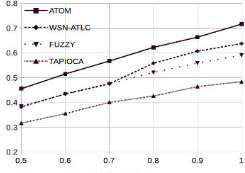
\includegraphics[width=\textwidth]{assets/159}
        \caption*{а)}
    \end{minipage}
    \hfill
    \begin{minipage}{0.45\textwidth}
        \centering
        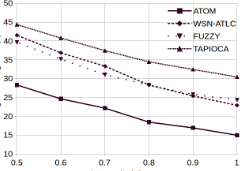
\includegraphics[width=\textwidth]{assets/160}
        \caption*{б)}
    \end{minipage}
    
    \vspace{10pt} % Adjust vertical spacing between rows

    \begin{minipage}{0.45\textwidth}
        \centering
        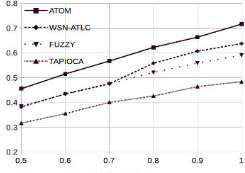
\includegraphics[width=\textwidth]{assets/159}
        \caption*{в)}
    \end{minipage}
    \hfill
    \begin{minipage}{0.45\textwidth}
        \centering
        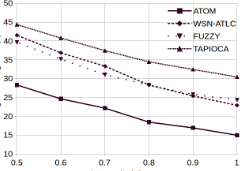
\includegraphics[width=\textwidth]{assets/160}
        \caption*{г)}
    \end{minipage}

\caption*{\bfseries 2-сурет. (а) қызмет көрсету жылдамдығы, (б) орташа күту уақыты,
(в) жасыл шамның жануын күту кезінде тоқтаған көліктердің орташа саны,
және (г) олардың қалыпты жүру жылдамдығы}

\end{figure}




\emph{Бір жолға 5 жолақты желілік желі}

Біз жолдардың санын және әрбір жол сегментінің ұзындығын сәйкесінше 800
м-ге дейін ұлғайту арқылы электр желісін ұлғайттық. 3-суретте нәтижелер
көрсетілген. Осы қондырғыдағы жолдың ені мен ұзындығының ұлғаюын ескере
отырып, 2 жолақты тор желісіне ұқсайтын жол кептелісі деңгейлерін
модельдеу үшін 0,6-дан 1,4-ке дейін таңдалады. 2 жолақты желіге
қарағанда 5 жолақты желілік желіде қызмет көрсетудің жоғары
көрсеткіштерін көрсетеді. Өткізу қабілеттілігінің артуын ескере отырып,
тиімділігі фазаны салыстыру үшін екі жолақты таңдаудың шектелуіне
байланысты төмендейді, бұл оның кеңейтілген жол желісіндегі қызмет
көрсету жылдамдығын төмендетеді. Тұтастай алғанда, АБОТ осындай үлкен
жолды орнату үшін өнімділікті айтарлықтай жақсартады, базалық
көрсеткіштер бойынша салыстырғанда 0,6-дан 1,4-ке дейін өседі. 3(а)
суреттегі нәтижелер ІРІ жол желілері үшін АБОТ-тың масштабталуын
көрсетеді.

\begin{figure}[H]
    \centering
    \begin{minipage}[b]{0.45\textwidth}
        \centering
        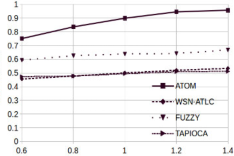
\includegraphics[width=\textwidth]{assets/161}
        \caption*{а)}
    \end{minipage}
    \hspace{0.05\textwidth} % Horizontal space between the figures
    \begin{minipage}[b]{0.45\textwidth}
        \centering
        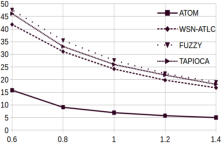
\includegraphics[width=\textwidth]{assets/162}
        \caption*{б)}
    \end{minipage}
    
    \vspace{0.05\textwidth} % Vertical space between rows of figures
    
    \begin{minipage}[b]{0.45\textwidth}
        \centering
        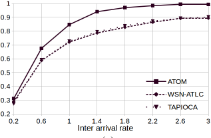
\includegraphics[width=\textwidth]{assets/163}
        \caption*{в)}
    \end{minipage}
    \hspace{0.05\textwidth}
    \begin{minipage}[b]{0.45\textwidth}
        \centering
        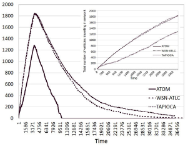
\includegraphics[width=\textwidth]{assets/164}
        \caption*{г)}
    \end{minipage}
\caption*{\bfseries 3-сурет. АБОТ өнімділігін бір жолға 5 жолақты желілік желіде
салыстыру (а) қызмет көрсету жылдамдығы, (б) орташа күту уақыты, (в)
тоқтатылған көліктердің орташа саны және (г) қалыпты жүргізу жылдамдығы }
\end{figure}


 

Бағдаршамның бағытталған жұмысы сигнал беру уақытын анықтау кезінде бір
немесе бірнеше қиылыстар қарастырылатынына байланысты екі санатқа бөлуге
болады. Бір қиылысу үшін мақсат жасыл сигналды оңтайлы жоспарлау болып
табылады. Мысалы traf C жарық реттегіші қиылыста келе жатқан көліктердің
баратын соңғы нүктесі аңықталады; жасыл шамды жоспарлаудың екі
стратегиясы ұсынылады, атап айтқанда, орташа күту/жол жүру уақытын
қысқарту мақсатында межелі жерге дейінгі аз орташа қашықтық болады. Екі
тәсіл де негізінен нақты уақыт режиміндегі трафикке негізделген
қашықтықтың кешігуін азайтуға бағытталған. Сонымен қатар, бүкіл сапар
барысында аялдамалардың жалпы санын азайтуға және осылайша
шығарындыларын азайтуға бағытталған.

Мақалада traf C реттеу кезінде бірнеше көршілес бөлімдер қарастырылды.
Мысалы, ережеге негізделген вертикалды дайындалған, көршілес
қиылыстардың қозғалыс шамдары жергілікті деңгейде үйлестірілген. Жұмыс
кеңейтілген {[}11,12{]} аймақтық деңгейде қосымша иерархиялық
бақылаушы/контроллер компоненті ұсынылды. Сонымен қатар, traf C жарық
жүйелеріне көп агент негізіндегі алгоритмдер қолданылды {[}13{]}. IEEE
802.15.4 технологиясы мен динамикалық фазалары арқылы өзара байланысқан
және бұрылыстарды факторинг кезінде жасыл уақытты есептейтін бірнеше
анық емес логикалық контроллерлерді пайдалану жолдары анықталды. Тraf C
көлемінің өзгеруін бақылау үшін сенсорларды пайдаланады, соның негізінде
олар бөлінген көп агентті жүйені пайдаланып N\textsubscript{d} көлік
құралының жүру кезіндегі ең қысқа жасыл шамдар, қиылыстарда күту уақыты
бойынша азайтылады. Көп агентті арматураны оқыту алгоритмдері {[}14{]}
пайдаланып, мұнда жергілікті және жақын қиылыстардың реакциялары traf C
шамдарының уақытын реттеу үшін қарастырылады, бұл тәсілдер жоғары
есептеу күрделілігін қажет етіп қабылдайды.

Бұл мақалада біз нақты уақыт режимінде жиналған қозғалыс жағдайын ескере
отырып, мақсатты қиылыстағы бағдаршам шамдарын бақылау арқылы сигналдың
максималды жылдамдығын арттыруға тырыстық. Біз жол желісін gd (V; E)
бағытталған графигі арқылы желісі ретінде ұсынамыз, мұндағы V
қиылыстарды қамтиды, яғни, E жол сегменттерінен, яғни арасындағы
бағытталған жиектерден тұрады. G негізінде біз бақыланатын бағдаршамды
ұсынамыз.

Қиылыстағы көліктердің қозғалыс бағытын біле отырып, төрт бағыттың
әрқайсысынан i-ге қанша көлік кіретінін? Мысалы, 4(b) суретте
көрсетілген i-ге кіретін 12 көліктің ішінде жеті көлік i-ге қарай жүруі
керек деп болжануда.

\begin{figure}[H]
	\centering
	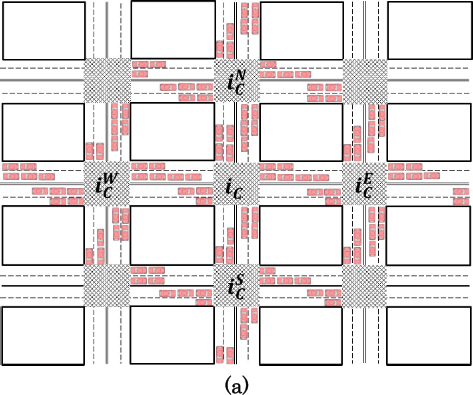
\includegraphics[width=0.4\textwidth]{assets/165}
	\caption*{}
\end{figure}

\begin{figure}[H]
	\centering
	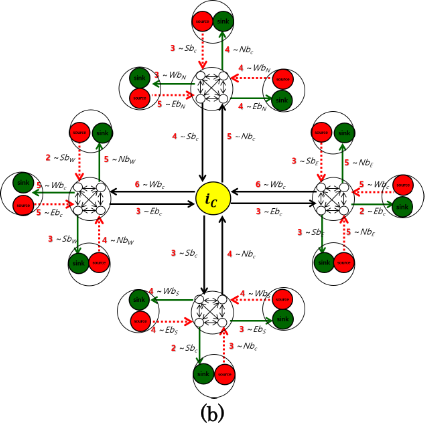
\includegraphics[width=0.4\textwidth]{assets/166}
	\caption*{}
\end{figure}

\begin{figure}[H]
	\centering
	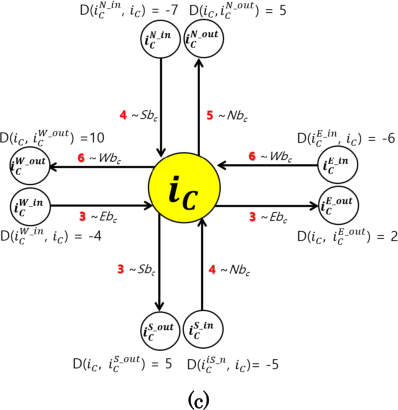
\includegraphics[width=0.4\textwidth]{assets/167}
	\caption*{}
\end{figure}

{\bfseries 4-сурет. Қиылыстағы көліктердің қозғалыс бағыттары}

TFM максималды бүтін санға дейін азайтылуы ағынының проблемасы шешіледі.
Оң жақ қиылыстағы қозғалыс ағынын бағытталған график түрінде ұсынылған
ағындық желіге салыстыруға болады. GD (V,E), V және E-қиылыстар
арасындағы қиылыстар мен жол сегменттерінің жиынтығы, тиісінше, (b)
тармағында көрсетіледі. (С) бөлігінде V-2-V кіретін Немесе шығатын
қозғалыс көлемі, Сондай-ақ әрбір 2 жол сегментінде жасыл шамды күтетін
қозғалыс көлемі қосымша көрсетіледі.

\emph{Зерттеу нәтижелерін талқылау.} Тraf C жарық фазасы мен ұзақтығын
реттеу арқылы i-ге байланысты көліктің жалпы Traf C көлемін барынша
арттыруға тырысады. Біз жаяу жүргіншілерді қарастырмайтындықтан,
оңтайландыру процедурасы жаяу жүргіншілердің i-де жолдарды кесіп өтуі
үшін ең аз жасыл уақытты есептемейді.

Сонымен қатар, автомобиль жүргізушілерге арналған көліктерді, сондай-ақ
өзін-өзі басқаратын көліктерді қарастырады; біріншісі үшін жеке көліктің
қозғалыс бағытын жүргізуші әр қиылыста, мысалы, v2i технологияларын
пайдалану арқылы немесе жүргізушінің ұялы телефонындағы қолданба арқылы
қамтамасыз етеді деп болжанады.

{\bfseries Қорытынды.} Бұл мақалада біз бағдаршам, жаңа traf c басқару
алгоритмін ұсындық. Адаптивті басқару әрбір қиылыста кіретін с уақыт
көлемі есептелінді, сонымен қатар көлік құралдарының әрбір уақыт үшін
келесі жол сегментінің кептеліс жағдайы тандалды. Содан кейін бағдаршам
traf c жарық фазаларын және олардың ұзақтығын көрші қиылыстармен бірлесе
отырып реттейді. Сонымен қатар, тәжірибеге үлестірілген немесе
орталықтандырылған түрде қолдануға болады. Нақты жол желілерін қолдана
отырып, ауқымды модельдеу тәжірибелері арқылы тексеріледі. Модельдеу
нәтижелері жол өткізу қабілеттілігін, көлік құралын күтудің орташа
уақытын және бәсекелес схемаға сәйкес көлік аялдамаларының орташа санын
жақсартатынын көрсетті. Негізінде, көбірек көліктердің жол желісі арқылы
өтуіне мүмкіндік береді және олардың жүру уақытын қысқартады, бұл тіпті
жоғары кептеліс жағдайында да көбірек көліктердің қозғалуына
көмектеседі. Осылайша, мұндай қондырғыдағы жолдың әртүрлі кептеліс
жағдайларында айқын өнімділігі оның тиімділігіне әсер етеді және іс
жүзінде тиімді екендігінің нақты дәлелі ретінде қарастырылады.

{\bfseries Әдебиеттер}

1. Бадагуев Б.Т. Эксплуатация транспортных средств (организация и
безопасность движения). -- М.: Альфа-Пресс, 2012. -- 240 с. ISBN
978-5-94280-556-2

2. Дудко Н.И., Петровец В.Р., Бершадский В.Ф. Безопасность движения
механических транспортных средств: пособие -- Горки: БГСХА, 2014. -- 237
с. ISBN 978-985-467-490-2

3. Блинкин М.Я. Безопасность дорожного движения: история вопроса,
международный опыт, базовые институции. -- М.: Изд. дом Высшей школы
экономики, 2013. -- 240 с. ISBN: 978-5-7598-1086-5

4. Волков В.С. Электрооборудование транспортных и
транспортно-технологических машин: учебное пособие -- М.: Академия,
2010. -- 208 с. ISBN 978-5-7695-5749-1

5. Горев, А. Э.Основы теории транспортных систем: учебное пособие / А.
Э. Горев; СПбГАСУ. -- СПб., 2010. -- 214 с. ISBN 978-5-9227-0266-9

6. Майборода М.Е., Беднарский В.В. Грузовые автомобильные перевозки. --
М.: Феникс, 2008. -- 442 с. ISBN 978-5-222-14364-3

7. Клинковштейн Г.И. Организация дорожного движения: учебник для вузов.
-- 5-е изд., перераб. и доп. -- М: Транспорт, 2001 -- 247. ISBN
9785277022405

8. Урыков В.А., Зеленина Л.И. Модели транспортного инфраструктурного
комплекса // https://web.snauka.ru/issues/2014. 18.06.2020.

9. Морозов И.И. и др. Численное исследование транспортных потоков на
основе гидродинамических моделей // Компьютерные исследования и
моделирование. -- 2011. -- Т. 3, №4. -- С. 389-412.

10. Буслаев А.П., Новиков А.В., Приходько В.М. и др. Вероятностные и
имитационные подходы к оптимизации автодорожного движения. -- М.: Мир,
2003. -- 368 с. ISBN 9785030036465

{\bfseries References}

1. Badaguev B.T. Jekspluatacija transportnyh sredstv (organizacija i
bezopasnost\textquotesingle{} dvizhenija). -- M.:
Al\textquotesingle fa-Press, 2012. -- 240 s. ISBN 978-5-94280-556-2
{[}in Russian{]}

2. Dudko N.I., Petrovec V.R., Bershadskij V.F.
Bezopasnost\textquotesingle{} dvizhenija mehanicheskih transportnyh
sredstv: posobie -- Gorki: BGSHA, 2014. -- 237 s. ISBN 978-985-467-490-2
{[}in Russian{]}

3. Blinkin M.Ja. Bezopasnost\textquotesingle{} dorozhnogo dvizhenija:
istorija voprosa, mezhdunarodnyj opyt, bazovye institucii. -- M.: Izd.
dom Vysshej shkoly jekonomiki, 2013. -- 240 s. ISBN: 978-5-7598-1086-5
{[}in Russian{]}

4. Volkov V.S. Jelektrooborudovanie transportnyh i
transportno-tehnologicheskih mashin: uchebnoe posobie -- M.: Akademija,
2010. -- 208 s. ISBN 978-5-7695-5749-1 {[}in Russian{]}

5. Gorev, A. Je.Osnovy teorii transportnyh sistem: uchebnoe posobie / A.
Je. Gorev;SPbGASU. -- SPb., 2010. -- 214 s. ISBN 978-5-9227-0266-9 {[}in
Russian{]}

6. Majboroda M.E., Bednarskij V.V. Gruzovye
avtomobil\textquotesingle nye perevozki. -- M.: Feniks, 2008. -- 442 s.
ISBN 978-5-222-14364-3 {[}in Russian{]}

7. Klinkovshtejn G.I. Organizacija dorozhnogo dvizhenija: uchebnik dlja
vuzov. -- 5-e izd., pererab. i dop. -- M: Transport, 2001 -- 247. ISBN
9785277022405

8. Urykov V.A., Zelenina L.I. Modeli transportnogo infrastrukturnogo
kompleksa // https://web.snauka.ru/issues/2014. 18.06.2020. {[}in
Russian{]}

9. Morozov I.I. i dr. Chislennoe issledovanie transportnyh potokov na
osnove gidrodinamicheskih modelej // Komp\textquotesingle juternye
issledovanija i modelirovanie. -- 2011. -- T. 3, №4. -- S. 389-412.
{[}in Russian{]}

10. Buslaev A.P., Novikov A.V., Prihod\textquotesingle ko V.M. i dr.
Verojatnostnye i imitacionnye podhody k optimizacii avtodorozhnogo
dvizhenija. -- M.: Mir, 2003. -- 368 s. ISBN 9785030036465 {[}in
Russian{]}

\emph{{\bfseries Авторлар туралы мәліметтер}}

Жаманғарин Д.С. -- PhD , Қ.Құлажанов атындағы ҚазТБУ, Астана, Қазақстан,
e-mail: Dus\_man89@mail.ru;

Алтынбек С.А. - PhD, Қ.Құлажанов атындағы ҚазТБУ , Астана, Қазақстан,
e-mail: Asa@mail.ru;

Тулегулов А.Д. - физика-математика ғылымдарының кандидаты,
қауымдастырылған профессор, Қ.Құлажанов атындағы ҚазТБУ, Астана,
Қазақстан, e-mail: tad62@ya.ru;

Акишев К.М.-техника ғылымдарының кандидаты, қауымдастырылған профессор,
Қ. Құлажанов атындағы ҚазТБУ, Астана, Қазақстан, e-mail:
akmail04@mail.ru;

Сапарходжаев Н.П. --Д. Серікбаев атындағы Шығыс Қазақстан техникалық
университеті, Өскемен, Қазақстан.

\emph{{\bfseries Information about the auhtors}}

Zhamangarin D.S. -- PhD, KazUTB named after K. Kulazhanov, Astana,
Kazakhstan, e-mail: Dus\_man89@mail.ru;

Altynbek S.A. - PhD, KazUTB named after K. Kulazhanov, Astana,
Kazakhstan, e-mail: Asa@mail.ru;

Tulegulov A.D. -- Candidate of Physical and Mathematical Sciences,
Associate Professor, KazUTB named after K. Kulazhanov, Astana,
Kazakhstan, e-mail: tad62@ya.ru;

Akishev K.M. - Candidate of Technical Sciences, Associate Professor,
KazUTB named after K. Kulazhanov, Astana, Kazakhstan, e-mail:
akmail04@mail.ru;

Saparkhodjaev N.P. - EKSTU. Ust-Kaman. Kazakhstan Astana, Kazakhstan.


